\chapter{Development Tools}
\label{appendix:dev-tools}

For the entire period of the doctoral studies, a multitude of programming applications and numerical software was used, adopted, and implemented in order to facilitate the research process and achieve the desired results.

\begin{description}
    \item[Writing language] The thesis and all of the papers were written using the \LaTeX {} language \cite{lamport1986latex}. This document was typeset using the TeXLive distribution for macOS \cite{texlivemacos}.
    \item[Editing software] Even though \LaTeX {} was adopted as the typeset language, the environment for writing the content itself was chosen to be \textbf{Visual Studio Code} \cite{vscode}. In fact, VS Code was also the main editor for most of the numerical methods developed for each objective of the conducted research.
    \item[Programming Languages] Testing the formalisms that were employed throughout the papers required lots of numerical algorithms (e.g., fitting procedures, differential equations, integrating functions). As a result, most of the work performed by the student was to develop code in different programming languages with the main goal of obtaining some results.
    \begin{enumerate}
        \item \texttt{Wolfram Mathematica} \cite{WolframMathematica} - used to perform calculus of differential equations, integrals and much more. For example, the classical energy functions for $^{163}$Lu were numerically evaluated using this application.
        \item \texttt{C++} - used to develop customized fitting procedures (e.g., the excitation energies for $^{163}$Lu). The implementations adopted newer standards, such as \texttt{C++11} and \texttt{C++14}.
        \item \texttt{Python} - this well-known programming language was heavily used for solving numerical equations, finding minima of various functions, but also double-checking the consistency of the other implementations done in \texttt{Mathematica} or \texttt{C++}. Only the version \texttt{python3} was utilized with modules such as \texttt{numpy, scipy}.
    \end{enumerate}
    The pie-chart shown in Fig. \ref{programming-languages-model} shows a proportion of the three languages adopted to implement the numerical algorithms. 
        \begin{figure}
            \centering
            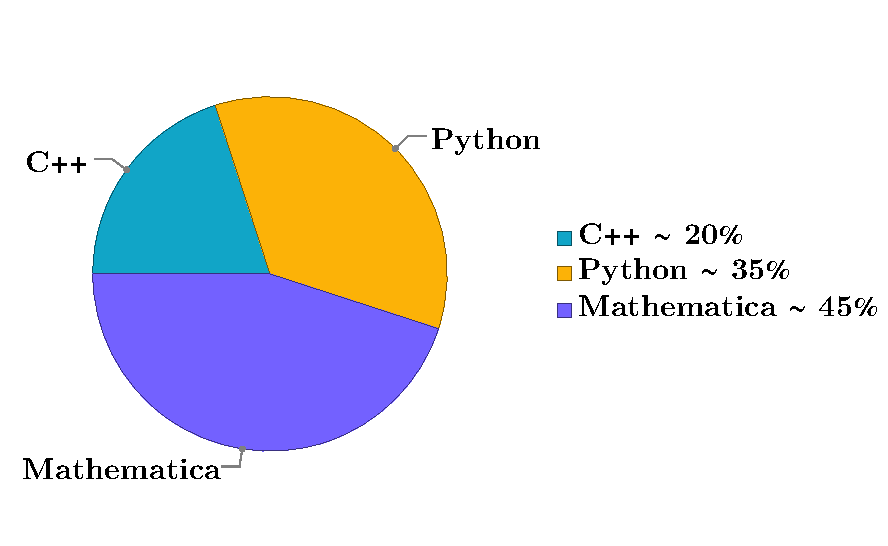
\includegraphics[scale=0.85]{Chapters/Figures/pieChartLanguages.pdf}
            \caption{Programming languages used to test all the formalisms that were developed during the doctoral studies.}
            \label{programming-languages-model}
        \end{figure} 
    \item[Drawing Tools] - Most of the graphical representations that were shown here were created using \texttt{Wolfram Mathematica}, as it provides a great suite of plot tools. Besides this, several plots were created with the \texttt{matplotlib} package \cite{Matplotlib} available in \texttt{Python}. Many diagrams were obtained by using \texttt{Libre Draw} \cite{LibreOffice} application, which also helped to enrich raw figures exported from \texttt{matplotlib} or \texttt{Mathematica}. Another great online tool used to generate workflow schemes was \texttt{Diagrams.net} \cite{diagrams.net}.
    \item[Source code] - Almost all of the algorithms were developed using \emph{version control} \cite{Git}, and the code is \textbf{open-source} (e.g., anyone can inspect, review, or contribute to the codebase) and available on \href{https://github.com/}{GitHub}. A few noteworthy repositories are given below:
    \begin{enumerate}
        \item Work on the odd-$A$ Lu isotopes - \href{https://github.com/basavyr/163Lu-New-TSD4-Formalism}{GitHub Repository}
        \item Results for $^{135}$Pr - \href{https://github.com/basavyr/pr135_EnergyFit_TW1TW2}{GitHub Repository}
        \item Classical Energy functions for $^{135}$Pr and $^{163}$Lu using Mathematica - \href{https://github.com/basavyr/mathematica-useful-algorithms}{GitHub Repository}
        \item Development of the $\mathbf{W_2}$ formalism - \href{https://github.com/basavyr/SymmetryPartners-RJP}{GitHub Repository}
    \end{enumerate}
\end{description}


